\chapter{Theoretische Grundlagen}\label{chap:relatedwork}
\fontsize{11}{12}\selectfont\begin{quote}„Process Mining ist eine vergleichsweise junge Wissenschaftsdisziplin, angesiedelt zwischen Computational Intelligence und Data Mining auf der einen Seite und Prozessmodellierung und Analyse auf der anderen. Die Grundidee von Process Mining ist es, reale Prozesse (im Gegensatz zu vermuteten oder angenommenen Prozessen) durch Extrahieren von Wissen aus EreignisEventlogs heutiger (Informations-)systeme zu erkennen, zu überwachen und zu verbessern.(...) 

Mit Hilfe von Methoden des Process Mining können Einsichten aus Ereignisdaten gewonnen werden, welche heutzutage in vielen Informationssystemen anfallen. Diese Methoden eröffnen neue Möglichkeiten, um Prozesse in einer Vielzahl von Anwendungsszenarien zu erkennen, zu überwachen und zu verbessern.“

- Process Mining Manifest \cite{PMManifesto}\end{quote}
\section{Prozessorientierte Datenanalyse}
Process Mining ist als Antwort auf die wachsende Nachfrage der Industrie entstanden, mehr Informationen über Prozesse, die sich im Unternehmens- und Produktionsalltag abspielen, verarbeiten, analysieren und zur Optimierung nutzen zu können. Es kann als technoEventlogisches Forschungsgebiet verstanden werden, das an dem Schnittpunkt zwischen Process Modelling und der Process Analysis sitzt und gemeinsame Merkmale mit den Bereichen des Data Mining und Machine Learning teilt, Vgl.\cite{Ailenei}.

Im Zuge der Digitalisierung in der Wirtschaftswelt hat auch das Erfassen und Speichern von kleinteiligen Informationen in zahlreichen Geschäftszweigen Einzug erhalten. Während das Sammeln von Daten aufgrund des informationstechnoEventlogischen Fortschritts kostengünstig geworden ist und sich mit wenig Aufwand implementieren lässt, ist die Auswertung der gesammelten Datenmengen für Unternehmen weiterhin ein resourcen- und zeitintensives Unterfangen. 
Eine rein statistische Analyse kann nur einen kleinen Teil der Informationen aufdecken, die sich hinter den erfassten Daten verbergen. Da diese Informationen von bedeutendem wirtschaftlichem Nutzen sein können, ist das Interesse an TechnoEventlogien, die das Problem der Auswertung lösen, groß.

Eine TechnoEventlogie die sich mit dieser Aufgabe befasst ist das Data Mining. Process Mining kann hierbei als Spezialgebiet des Data Minings aufgefasst werden, dessen Einsatz immer dann sinnvoll ist, wenn die gesammelten Rohdaten, über die man mehr erfahren möchte, in einem zeitlichen Kontext miteinander in Verbindung stehen und einen Prozess beschreiben.
Process Mining Modelle unterscheiden sich von traditionelleren Sequenz Mining Methoden wie Hidden Markov Modellen\cite{hmm} und Recurrent Neural Networks\cite{rnn} dadurch, dass sie visuell dargestellt werden können und ihre visuelle Darstellung für eine einfache und direkte Kommunikation zwischen prozessbeteiligten Stakeholdern genutzt werden kann, Vgl.\cite{localMining}.

Zusammenfassend betrachtet kann Process Mining als Werkzeug verstanden werden, welches eingesetzt wird, um Daten, die von den Informationssystemen in Form von Protokolldateien, im folgenden auch Eventlogs genannt, aufgenommen werden, auszuschöpfen. Es hat zum Ziel  Informationen über den den Daten innewohnenden Prozessablauf zu gewinnen, wie es auch im "Process Mining Manifest", das von der IEEE Task Force on Process Mining 2011 veröffentlicht wurde, beschrieben wird \cite{PMManifesto}. 

Protokolldateien allein sind, insbesondere wenn sie unsystematisch in großen Mengen erfasst wurden, nur durch manuelle Nachverarbeitung in der Lage Antworten auf prozessrelevante Fragen zu liefern. Die Antwort auf Fragen danach, wie ein gewöhnlicher Arbeitsablauf aufgebaut ist, wann es an welchen Stellen zu Abweichungen kommt und wodurch diese provoziert werden, oder wie ein verbesserter Ablauf gestaltet werden könnte, liegt meist in diesen Informationen eingebettet. Die in der Protokolldatei verankerten Daten dienen dem Process Mining dazu die entsprechenden Antworten systematisch aufzudecken. 

Beim Process Mining wird zwischen drei unterschiedlichen Funktionen unterschieden:  \textit{discovery, conformance} and \textit{enhancement}, also dem Entdecken, Einhalten und Optimieren von Prozessen, siehe Abbildung \ref{fig:pm_functions}, Vgl.\cite{PMManifesto}.
\vspace{10mm}

\begin{figure}[!ht]
    \centering
    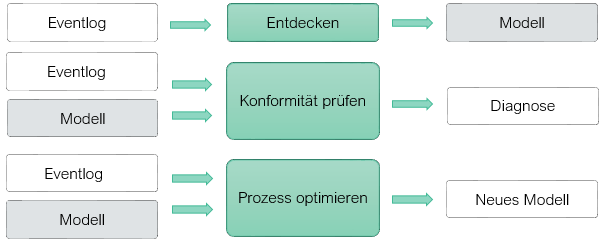
\includegraphics[scale=0.8]{figures/Appbildungen/PM_functions.PNG}
    \caption{Die drei Typen des Process Mining (Eigene Darstellung in Anlehnung an: Process Mining Manifest, 2011, S.4, \cite{PMManifesto})}
    \label{fig:pm_functions}
\end{figure}

\newpage
\subsection{Process Mining Typen}
Die drei unterschiedlichen Typen kennzeichenen folgende Eigenschaften und Abläufe:
\begin{itemize}
\item \textbf{Discovery}: Im Ausgangszustand besteht keinerlei a Priori Modell. Der Discovery Vorgang beschäftigt sich damit, den real geschehenden Prozess, anhand der von den verbundenen Geräten hinterlassenen Eventlogs, herauszukristallisieren und ein Prozessmodell aus der gegebenen Historie der Geschehnisse zu erstellen.

\item \textbf{Conformance Checking}: Konformität prüfen - Ein a-priori Modell des Prozesses existiert. Conformance Checking vergleicht den real existierenden Ablauf mithilfe des Eventlogs mit dem erwünschten Prozess um festzustellen, ob das beobachtete Verhalten mit dem geplanten Prozess übereinstimmt. Dieser Vorgang ermöglicht die Aufdeckung von Abweichungen zwischen geplanten und tatsächlichen Prozessvorgängen und kann auf Abweichungen hinweisen.  Conformance Checking schließt Compliance Checking mit ein, d.h. der beobachtete Prozess wird auch daraufhin untersucht, ob er sich an vorgefertigte Regeln, Spezifikationen oder relevante Normen hält.

\item \textbf{Enhancement}: Ein a-priori Modell des Prozesses existiert. Das Ziel ist die Optimierung oder Umgestaltung eines Modells, mithilfe der, aus der Auswertung des Eventlogs, gewonnenen Informationen. Ein Prozess kann nun in Bezug auf seine Performanz oder Einhaltung geforderter Standards hin verbessert oder erweitert werden. Informationen wie Kostenanalyse, Zeitaufwand oder Priorisierung einzelner Schritte können in die Optimierung miteinfließen, Engpässe die beobachtet  wurden können umgangen werden.
\end{itemize}

Ausgabe der Discovery Funktion und Grundlage für alle weiteren Schritte ist die Umwandlung des aufgenommenen Protokolls in ein graphisches Modell, in der Regel handelt es sich dabei um ein Petri Netz. Petri Netze sind eine methodische Darstellungsform, die dazu dient nebenläufige Prozesse zu beschreiben. Da Petri Netze auch im folgenden praktischen Teil der Arbeit eingesetzt werden, werden sie hier kurz erläutert. 

\subsection{Petri Netze}
Formell werden Petri Netze als gerichtete, bipartite Graphen definiert, die aus Stellen  und  Transitionen  bestehen und durch  gerichtete  Kanten  verbunden sind, wie sie in \textit{Software Engineering durch Modellierung wissensintensiver Entwicklungsprozesse} beschrieben sind \cite{freund2007software}. 

\begin{figure}[!h]
    \centering
    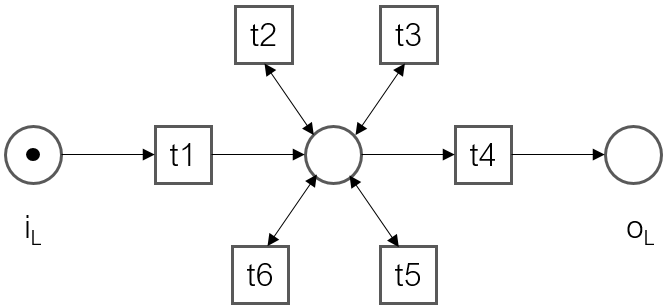
\includegraphics[width=0.65\textwidth]{figures/Appbildungen/petriNetFlower.png}
    \caption{Ein unmarkiertes Petri Netz mit Eingangsstelle $i_L$ und Ausgangsstelle $o_L$}.
    \label{fig:exampleFlower}
\end{figure}
Ein Petri-Netz wird formal durch das Tripel $N = (S, T, F)$ definiert. $S$ ist die Menge der Stellen, $T$  ist  die  zu  $S$  disjunkte  Menge  der  Transitionen  und  $F⊆ (S ×  T) ∪ (T  ×  S) $ ist  eine Flussrelation,  welche  die  Menge  der  Kanten  bezeichnet.  Die  Elemente  aus  $S$  werden grafisch repräsentiert durch Kreise, Elemente aus $T$ durch Rechtecke und Elemente aus $F$ als gerichtete Kanten zwischen Stellen und Transitionen. Stellen,  die  sich  vor  Transitionen  befinden, werden Eingangsstellen genannt, Stellen nach Transitionen sind deren Ausgangsstellen. 

$T$ ist eine endliche Menge von Übergängen für die gilt: $S ∩ T =  ∅.$

$F ⊆(S × T) ∪ (T × S)$ beschreibt eine zweistellige Relation.

Eine  Stelle  $s∈S$  ist  Eingabestelle  einer  Transition  $t∈T$,  wenn  eine  gerichtete  Kante  von $s$ nach $t$ existiert. Eine Stelle $s$ ist Ausgabestelle einer Transition $ t$, wenn eine gerichtete Kante von $t$ nach $s$ existiert. Die Menge aller Eingabestellen einer Transition t wird mit $\cdot t$ bezeichnet und Vorbereich genannt. Die Menge aller Ausgabestellen einer Transition $t$ wird mit $t \cdot$ bezeichnet und Nachbereich genannt.

Markierungen definieren die Semantik der Netze. Jede Stelle kann eine oder mehr Markierungen beinhalten, die illustriert als Punkt auf der jeweiligen Stelle markiert werden. Eine Transition kann aktiv werden, wenn auf jeder Stelle, von der aus eine Kante zu dieser Transition führt, mindestens eine solche Markierung liegt. Eine aktive Transition kann schalten, indem sie von allen Eingangsstellen eine Markierung entfernt und zu jeder Ausgangsstelle eine Markierung hinzufügt. Damit sind Transitionen aktive Einheiten und ermöglichen so die Darstellung der legitimen Aktivitäten eines Prozesses, Vgl. \cite{Petrinetze}.
\newpage
\subsection{Qualitätskriterien}\label{quality}
Für die Bewertung der Qualität eines Ausgabemodels  bedarf es fester Kriterien. Diese unterscheiden sich jedoch je nach Anwendungsfall gravierend in ihrer Bedeutung, da die Ansprüche an ein Ausgabemodell abhängig von der beabsichtigen Verwendung des Modells und der Zielgruppe sind, die das Modell zielführend interpretieren soll. In der Literatur werden meist folgende vier Dimensionen zur Beurteilung herangezogen \cite{PMinAction}:

\begin{itemize}
\item \textbf{Fitness}: Eine perfekte Fitness bedeutet, dass das Prozessmodell das Verhalten aus dem Eventlog vollständig wiedergibt. Sie beschreibt den Grad zu dem Prozesse in der Realität vom Modell abgedeckt werden.
 
\item \textbf{Precision}: ein Maß, das beschreibt, ob das Modell Verhalten erlaubt, das grundlegend verschieden vom im Eventlog aufgezeichneten Verhalten ist. Ein Modell mit geringer Präzision ist "unterformt". Das heißt es lässt sowohl Verhalten zu, dass sich aus dem Eventlog ergibt, als auch sehr viele weitere Ereignisketten. Dadurch ist die Aussagekraft des Modells niedrig. Es entsteht dabei ein sogenanntes Blumenmodell, bei dem von einer Transition aus viele Stellen beliebig oft erreichbar sind, entsprechend Abbildung \ref{fig:exampleFlower}.

\item \textbf{Generalization}: Die Generalisierung gibt an, in wie weit das Verhalten aus dem Eventlog im Ausgabemodell verallgemeinert wurde. Ein Modell soll generalisieren, dabei aber nicht das Verhalten welches in dem Eventlog vorhanden ist einschränken. Man sagt ein "überformtes" Modell generalisiert nicht genug - Abläufe die Teil des Modells sein sollten, werden nicht repräsentiert.

\item \textbf{Simplicity}: Die Komplexität des Ausgabemodells sollte auf das Nötigste reduziert werden. Dieses Attribut steht in einem engen Konflikt mit den anderen genannten Dimensionen. Ihr Maß sollte gemeinhin der Zielgruppe und dem Anwendungsfall angepasst werden. Ein Modell, das die Wirklichkeit akkurat wieder gibt, aber vom Anwender nicht interpretiert werden kann, erfüllt seinen Zweck nicht. Wird das Modell wiederum zu stark vereinfacht, können für den Anwender relevante Informationen ausgeblendet werden.
\end{itemize}

Da diese Dimensionen in einer Wechselbeziehung zueinander stehen und sich gegenseitig beeinflussen, ist es je nach Kontext notwendig sie gegeneinander abzuwägen. In vielen Fällen soll das Ausgabemodell ein möglichst detailgetreues Abbild des Verhaltens aus dem Eventlog nachbilden, also auch die Mehrzahl der auftretenden Muster wiedergeben. 
Es kann je nach Anwendungsfall auch wünschenswert sein, eine möglichst einfache und wenig komplexe Abstraktion aus dem Eventlog zu generieren, welches dann bewusst auf selten auftretende Muster  verzichtet und aus einer möglichst geringen Anzahl an Knoten und Kanten im Netz besteht. Diese Frage sollte vom Anwender des Process Mining beantwortet werden, bevor die Prozessanalyse beginnt.

\subsection{Herausforderungen}\label{challanges}
Process Mining kann nur dann aufschlussreiche Antworten auf Fragen nach Prozesstrukturen liefern, wenn die Daten, mit denen es arbeitet, vordefinierte Kriterien erfüllen. Wie in anderen Gebieten der Datenanalyse gilt auch hier das Prinzip \textit{Garbage in, Garbage out} \cite{GIGO}. 

\subsubsection{Rauschen}
Eine der größten Fehlerquellen des Process Mining ist Rauschen in den zur Verfügung stehenden Daten. Um ein Modell zu erzeugen, das möglichst wenig von dem reellen Prozess abweicht, muss angenommen werden, dass das Eventlog, welches als Input dient, alle reellen Vorgänge vollständig widerspiegelt. Wenn viele Einträge, relativ zur insgesamt erfassten Datenmenge gemessen, im Eventlog vorliegen, die irrelevant sind oder als Ausnahmesituation gewertet werden, wird der Process Mining Algorithmus nicht oder nur schlecht in der Lage sein, diese als Rauschen zu identifizieren. Es ist dann wahrscheinlich, dass fehlerbehaftete Muster erkannt werden, die dem realen Prozess nur teilweise entsprechen oder in gravierenden Fällen vollkommen widersprechen.

Ein Ansatz um Rauschdaten zu umgehen ist es systematisch Schwellwerte für ihre Auftrittshäufigkeit zu finden, so dass Rauschdatensätze herausgefiltert werden, bevor die eigentliche Analyse einsetzt. 

\subsubsection{Unvollständigkeit}
Sind zu wenige Daten vorhanden oder werden umfangreiche Prozesse nicht detailgetreu dokumentiert, kann Process Mining nicht garantieren, dass das resultierende Modell vollständig ist. 
Fehlende Informationen können manuell in der Vorverarbeitung der Daten nachgetragen werden, verlangsamen aber den Analyseprozess und sind fehleranfälliger als automatisiertes Sammeln und Eintragen von Informationen. 

Nicht nur Mangel an korrekt deklarierten Attributen, auch im Protokoll nicht dokumentierte Ereignisse, die aber im realen Ablauf essentiell für den Prozess sind, können dazu führen, dass ein Modell unvollständig ist. Eine weitere Fehlerquelle ist der umgekehrte Fall, wenn Einträge aufgezeichnet wurden, obwohl bestimmte Aktivitäten nicht stattgefunden haben. Beispielsweise im Vorfeld eingetragene Termine die nachträglich abgesagt wurden, ohne dies im System zu vermerken. 

Ein Prozesschritt kann auch unerkannt bleiben, obwohl er im Eventlog dokumentiert wird. Dies kann geschehen wenn die Dokumentation zu kleinschrittig bleibt, als dass erkannt werden kann, um welchen übergreifenden Prozesschritt es sich handelt. 

Um das Problem der Unvollständigkeit zu vermeiden, muss vor der Analyse sichergestellt werden, dass jede für den Prozess relevante Instanz automatisch Einträge im Eventlog generiert, sobald neue Aktionen eintreten und verhindert werden dass Einträge entstehen, die nicht der Realität entsprechen.

\subsubsection{Parallele Abläufe}
Die Einträge eines Eventlogs liegen stets in sequentieller Form vor, was das Aufdecken von parallel ablaufenden Vorgängen erschwert. Falls Anfang und Ende der Aktivitäten protokolliert werden, erleichtert dies die korrekte Modellierung. In den allermeisten Systemen werden Aktivitäten jedoch als atomare Vorkommnisse im Eventlog vermerkt. Dann muss in der Analyse, aus dem verschachtelten auftreten von Prozessen in einer Vielzahl von Einträgen, auf die Parallelität geschlossen werden. Liegen nur wenige Einträge vor, sinkt auch die Wahrscheinlichkeit, dass parallele Abläufe korrekt klassifiziert werden. Die Strategie mit der parallele Sequenzen von Process Mining Algorithmen erkannt werden, kann sich von Verfahren zu Verfahren stark unterscheiden und unterschiedlich zuverlässig ausfallen.

\subsubsection{Schleifen}
Ein weiteres Hindernis für Process Mining Algorithmen ist die korrekte Identifizierung von zyklischen Abläufen in einem Eventlog, besonders kurze Schleifen, bestehend aus nur einer oder zwei Aktivitäten, sind für einfache Process Mining Verfahren schwierig zu erkennen. 
Wenn der Protokollierungsmechanismus um die Funktion erweitert wird, zyklische Abläufe zu nummerieren, kann die korrekte Modellierung erleichtert werden. Diese Funktion kann aber nicht in jedem System als gegeben vorausgesetzt werden.

%Im Gegensatz zu Rauschdaten, die durch einen Fehlerhaften  Protokollierungsvorgang hervorgerufen werden, können Ausnahmefälle und fehlerhafte Instanzen für eine Evaluation des Prozesses von größerem Interesse sein, wenn der Andwendungsfall vorsieht Abweichungen zu einem organisierten Prozess zu entdecken. 

%Sie können für den Modellierungsprozess aber irrelevant sein, wenn das Ziel ist ein möglichst generisches Modell zu erzeugen, dann müssen die Ausreißer im Protokoll durch ausreichend korrekte Abläufe anteilsgemäß aufgehoben werden. 

%Der erfolgreiche Einsatz von Process Mining Algorithmen setzt außerdem voraus, dass der Prozess vom EreignisEventlog bis hin zur Interpretation des Modells begleitet wird von Personen, die sowohl mit den Stärken und Schwächen der Process Mining Methode vertraut sind, als auch den Eigenschaften der untersuchten Umgebung sowie den Einsatzzweck des Process Mining kennen und darüber hinaus wissen, wie gegebene Parameter des eingesetzten Verfahrens anzupassen sind, wie die Eingangsdaten aufbereitet werden müssen und wie weit die Aussagekraft des Ergebnismodells reicht. (entfernen?)
\section{Process Mining Algorithmen}
Die Grundlage für die allermeisten algorithmischen Verfahren zur Konstruktion von Prozessmodellen sind Ordnungsrelationen. Im Process Mining beschreiben sie die Beziehung, oder das fehlen einer Beziehung, zwischen zwei Elementen eines Prozesses. 
Als ein verbreitetes  Beispiel für ein rein algorithmisches Verfahren zur Prozessentdeckung, das auf Ordnungsrelationen basiert, kann der $\alpha$-Algorithmus genannt werden, dessen Ablauf unter Algorithmus \ref{alg:alphaminer} einzusehen ist.
Es handelt sich dabei um eine sehr einfache Variante eines Process Mining Algorithmus, der für wenig komplexe Eventlogs aber, nach den zuvor beschriebenen Qualitätskriterien, korrekte Modelle erstellen kann. Er soll hier als einleitendes Beispiel für Process Mining Discovery im Allgemeinen näher betrachtet werden. \newline

\providecommand\algorithmname{alphaminer}
\begin{algorithm}
  \caption{Alpha Miner}
  \label{alg:alphaminer}
  \begin{algorithmic}[1]
    \State $T_L = \{ t \in T \;\mid \exists_{\sigma \in L} \; t \in \sigma\}$ \label{op0}
    
    \State $T_I = \{ t \in T \;\mid \exists_{\sigma \in L} \; t=first(\sigma)\}$ \label{op1}
    
    \State $T_O = \{ t \in T \;\mid \exists_{\sigma \in L} \; t=last(\sigma)\}$ \label{op2}
    
    \State $X_L = \{ (A,B) \mid A \subseteq T_L \land A \neq $\o$ \land B \subseteq T_L \land B \neq $\o$ \land \forall_{a\in A} \forall_{b\in B}\; a \to _L b \land \forall_{a1,a2\in A} a_1 \# _L a_2 \land \forall_{b1,b2\in B} b_1 \# _L b_2\}$ \label{op3}
    
    \State $Y_L = \{ (A,B) \in X_L \mid \forall_{A',B' \in X_L} A \subseteq A' \land B \subseteq B' \implies (A,B) = (A',B')\}$ \label{op4}
    
    \State $P_L = \{ p_{(A,B)} \mid (A,B) \in Y_L \} \cup \{i_l, o_L \}$ \label{op5}
    
    \State $F_L = \{ (a,p_{(A,B)}) \mid (A,B) \in Y_L \land a \in A \} \cup \{  (p_ {(A,B)},b) \mid (A,B) \in Y_L \land b \in B \} \cup \{ (i_l,t \mid t \in T_I  \} \cup \{ (t,o_L \mid t\in T_o\}$ \label{op6}
    
    \State $\alpha(L) = (P_L, T_L, F_L) $ \label{op7}
    
  \end{algorithmic}
\end{algorithm}

Das Verfahren arbeitet mit verlaufsdatenbasierten Ordnungskriterien (Englisch \textit{Eventlog-based ordering relations}). Die kausale Beziehung zwischen Aktivitäten $(a→b)$ wird geschlossen, wenn zwei Aktivitäten $a$ und $b$ mindestens einmal in der Sequenz $(ab)$ im Eventlog vorkommen, und die Sequenz $(ba)$ nie auftritt. Auf parallele Ausführung zweier Aktivitäten $(a|b)$ wird durch die Verschränkung dieser Aktivitäten geschlossen. Auf die Unabhängigkeit zweier Aktivitäten $a$ und $b$ $(a\#b)$ wird geschlossen, wenn weder die Sequenz $(ab)$ noch die Sequenz $(ba)$ im Eventlog vorkommt.

Im ersten Schritt des Verfahrens werden alle Aktivitäten des Eventlogs in einer Menge zusammengefasst. In Schritt 2 und 3 des Algorithmus werden die Mengen der ersten und letzten Elemente aller Sequenzen in einer Menge gesammelt. 
Schritte 4 und 5 stellen den eigentlichen Kern des $\alpha$-Miner Algorithmus dar. Die Positionen und die Verbindungen der Elemente müssen systematisch ermittelt werden. Es sollen Knoten $p(A,B)$ der Art entstehen, dass $A$ die Menge der Übergangseingänge ist und $B$ die Menge der Übergangsausgänge. Alle Elemente der Menge $A$ sollen in einer kausalen Beziehung zu den Elementen der Menge $B$ stehen, die Elemente der Menge stehen dabei nicht in einer Beziehung zu Elementen der eigenen Menge.

In Schritt 6 werden außerdem die Knoten $i_L$ und $o_L$ festgelegt, dabei handelt es sich um die Anfangs- und Endknoten des zu konstruierenden Netzes, sie werden als \textit{Source} beziehungsweise \textit{Sink} bezeichnet. Schritt 7 des Algorithmus ist verantwortlich für die Erzeugung der Kanten des Netzes, entsprechend der Beziehung zwischen den Knoten, die durch eine Kante verbunden werden. Abschließend wird in Schritt 8 das gesamte Netz aus den zuvor bestimmten Netzkomponenten zusammengesetzt und der Algorithmus endet.
\newpage
\subsection{Beispiel einer Analyse einer Protokolldatei}
Das Ausgabemodell einer Process Mining Discovery Analyse über der selben Protokolldatei kann, in Abhängigkeit von der Strategie des eingesetzten Process Mining Verfahrens, variieren. Process Mining Algorithmen ähneln sich jedoch größtenteils in ihrer grundlegenden Struktur. Um den im vorangegangen Abschnitt vorgestellten Algorithmus verständlich zu machen, soll hier exemplarisch eine Auswertung durch den $\alpha$-Miner Algorithmus schrittweise nachvollzogen werden.

Da der Schwerpunkt dieser Arbeit auf dem Entdecken von Prozessen, also dem Process Mining Typ der \textit{ Discovery} liegt, werden im Rahmen dieser Arbeit Process Mining Verfahren betrachtet, die auf der Definition des 'General Process Discovery Problem' beruhen, zu Deutsch 'Problem der allgemeinen Prozessentdeckung', Vgl. Process Mining in Action, 2016, S.163 \cite{PMinAction}:
\begin{addmargin}[20pt]{20pt} 
Man betrachte ein Eventlog $L$ und eine Menge $A$ an Aktivitäten. Eine einfache Sequenz $\sigma$ sei eine Folge von Aktivitäten, sprich $\sigma ∈ A $. Ein Eventlog $L$ setzt sich zusammen aus mehreren Sequenzen über $A$, also ist $L ∈ B(A)$. Ein Process Discovery Algorithmus ist eine Funktion $\gamma$ die einen Input $L$ auf ein Prozess Modell derart abbildet, das es das aufgenommene Verhalten repräsentiert.
\end{addmargin}
Eine gute Repräsentanz ist dann gefunden, wenn die vier Qualitäten des Ausgabemodells (\textit{Fitness, Precision, Generalization, Simplicity}) ein für den Anwendungsfall akzeptables Gleichgewicht erreichen.

Man betrachte ein Eventlog der Form: $L = [(a, c, d)^6, (b, c, d)^5, (a, c, e)^4, (b, c, e)^2]$
Das Eventlog resultiert in der Ordnungsrelation, die in Tabelle \ref{tab:Ordnungsrelation} aufgeführt ist.
\begin{table}[!ht]
\centering
\resizebox{\columnwidth/3}{!}{%
\begin{tabular}{cccccc}
 & \textbf{a} & \textbf{b} & \textbf{c} & \textbf{d} & \textbf{e} \\ \cline{2-6} 
\multicolumn{1}{c|}{\textbf{a}} & \multicolumn{1}{c|}{\textit{\#}} & \multicolumn{1}{c|}{\textit{\#}} & \multicolumn{1}{c|}{→} & \multicolumn{1}{c|}{\textit{\#}} & \multicolumn{1}{c|}{\textit{\#}} \\ \cline{2-6} 
\multicolumn{1}{c|}{\textbf{b}} & \multicolumn{1}{c|}{\textit{\#}} & \multicolumn{1}{c|}{\textit{\#}} & \multicolumn{1}{c|}{→} & \multicolumn{1}{c|}{\textit{\#}} & \multicolumn{1}{c|}{\textit{\#}} \\ \cline{2-6} 
\multicolumn{1}{c|}{\textbf{c}} & \multicolumn{1}{c|}{\textit{←}} & \multicolumn{1}{c|}{\textit{←}} & \multicolumn{1}{c|}{\#} & \multicolumn{1}{c|}{\textit{→}} & \multicolumn{1}{c|}{\textit{→}} \\ \cline{2-6} 
\multicolumn{1}{c|}{\textbf{d}} & \multicolumn{1}{c|}{\textit{\#}} & \multicolumn{1}{c|}{\textit{\#}} & \multicolumn{1}{c|}{←} & \multicolumn{1}{c|}{\textit{\#}} & \multicolumn{1}{c|}{\textit{\#}} \\ \cline{2-6} 
\multicolumn{1}{c|}{\textbf{e}} & \multicolumn{1}{c|}{\textit{\#}} & \multicolumn{1}{c|}{\textit{\#}} & \multicolumn{1}{c|}{←} & \multicolumn{1}{c|}{\textit{\#}} & \multicolumn{1}{c|}{\textit{\#}} \\ \cline{2-6} 
\end{tabular}%
}
\caption{Ordnungsrelation zu einem Eventlog $L$ auf Basis des $\alpha$-Miner Verfahrens}
\label{tab:Ordnungsrelation}
\end{table}
\newline
Da auf Aktivität $a$ $b$ folgt, aber auf $b$ nie $a$ folgt, besteht die kausale Beziehung $(a→b)$ und man erwartet, dass ein Modell diese Beziehung reflektiert.

Die Relationsmatrix aus Tabelle \ref{tab:Ordnungsrelation} lässt sich auch als Menge wie folgt darstellen:

$ X_L={ [({a}, {b}), ({a}, {c}), ({a}, {e}), ({a}, {b, e}),
({a}, {c, e}), ({b}, {d}), ({c}, {d}), ({e}, {d}),
({b, e}, {d}), ({c, e}, {d}) ]}$

Wenn ein Knoten für jedes Element der Menge entstünde, würde die Anforderung der Generalisierung verletzt werden. Aus diesem Grund wird eine Bedingung „Maximales Pair“ $(A,B)$ definiert und die Elementmenge gefiltert, konkret werden alle redundanten Elemente der Menge der Länge zwei entfernt. Es entsteht:

$ X_L={ [({a}, {b, e}), ({a}, {c, e}),
({b, e}, {d}), ({c, e}, {d}) ]}$

Nach Ausführung aller Schritte des $\alpha$-Miners auf das Eventlog $L$ entsteht folgendes Petri Netz:

\begin{figure}[!h]
    \centering
    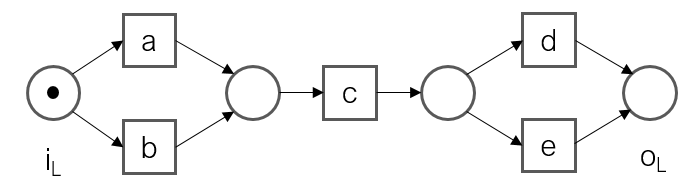
\includegraphics[scale=0.65]{figures/Appbildungen/alpha_petri_net.png}
    \caption{Petri Netz, Resultat des Alpha Miner Verfahrens}
    \label{fig:petriNetExample}
\end{figure}

Der $\alpha$-Miner Algorithmus ist aufgrund seines simplen Aufbaus nicht in der Lage, jede Prozessfolge korrekt zu identifizieren und zu modellieren, beispielsweise werden parallele Abläufe und kurze Schleifen nur unzureichend erkannt.

Um die Probleme in der Prozessanalyse zu bewältigen und Process Mining verschiedenen Anforderungen gegenüber anzupassen, sind im Laufe der Jahre eine Reihe an fortgeschrittenen Algorithmen entwickelt worden, die für unterschiedliche Anwendungsfälle jeweils eigene Vor- oder Nachteile mitbringen können. 

Ein Beispiel für einen Algorithmus der auf der Basis vom Alpha Miner entwickelt wurde ist der Heuristic Process Miner.

\subsection{Heuristic Process Miner}
Der Heuristic Miner basiert auf den Grundlagen des $\alpha$-Miner, arbeitet aber mit zusätzliche Kriterien, die beim Erzeugen des Modells berücksichtigt werden. Wie der Name des Verfahrens vermuten lässt, nutzt der Miner eine Heuristik um zu bewerten, welche Abfolgen tatsächlich Teil des resultierenden Modells werden sollten, konkret wird hierfür die Häufigkeit von Nachfolgerelationen berücksichtigt, Vgl.\cite{heurMining}.

Das Verfahren unterscheidet sich kaum von der Vorgehensweise des $\alpha$-Miners, allerdings wird statt allein zu unterscheiden, ob eine direkte Folge zwischen zwei Knoten besteht oder nicht, eine Beziehung zwischen zwei Elementen $a$ und $b$ über einen numerischen Wert gewichtet. Das Gewicht der Kante entspricht der Relevanz der Folgebeziehung im Modell. Das Gewicht der Kante wird berechnet über die Formel: 
\begin{equation}
 {a} \Rightarrow _L {b} = \left(\frac{ | {a} >_L {b} - {b} >_L {a} }{|{a} >_L {b}| + |{b} >_L {a}| + 1 }\right)
 \end{equation}
 Dabei beschreibt $|{a} >_L {b}|$ die Häufigkeitsmenge, mit der $b$ auf $a$ in $L$ folgt, wobei $L$ das Eventlog über der Menge der Protokolleinträge darstellt. Die berechneten Werte liegen zwischen 1 und -1, Werte um den Bereich Null deuten auf darauf hin, dass zwei Einträge unabhängig sind, positive Werte nahe 1 deuten auf eine Abhängigkeitsbeziehung hin, negative auf eine Abhängigkeitsbeziehung in umgekehrter Richtung, also gilt:
 \begin{equation}
 {a} \Rightarrow _L {b} =  -1 \cdot ( {b} \Rightarrow _L{a} )
 \end{equation}
Schleifen der Länge eins stellen bis hier hin weiterhin ein Problem für das Verfahren dar, da die Kante von einem Knoten a zu sich selbst mit niedrigen Werten Gewichtet wird. Um dies zu umgehen wird eine Abwandlung der Formel (1) für kurze Schleifen eingeführt:
 \begin{equation}
 {a} \Rightarrow _L {a} = \left(\frac{ | {a} >_L {a}}{
|{a} >_L {a}| + 1 }\right)
 \end{equation}
Anhand dieser Formel kann eine Relationstabelle, entsprechend der Tabelle \ref{tab:Ordnungsrelation} in der Einführung, angelegt werden. Der Heuristics Miner nutzt aber statt der symbolischen Werte, die zwischen vier Zuständen unterscheiden, nun das Gewicht der zugehörigen Kanten. 

Als nächstes berechnet das Verfahren drei Schwellwerte, die jeweils dazu dienen, Rauschen von relevanten Daten zu unterscheiden. Der Schwellwert dient dazu zu entscheiden, ob es sich bei einem Eintrag um Ausreißer in der Datenmenge, oder aber um sporadische, aber für das Modell entscheidende, Ereignisse handelt. Abschließend wird basierend auf diesen Berechnungen ein Modell generiert.

Der Heuristics Miner kann im Gegensatz zum $\alpha$-Miner auch kurze und lange Schleifen korrekt wiedergeben, muss aber mit zusätzlichen Metriken arbeiten um sogenannte\textit{ long distance dependencies}, also Abhängigkeiten in großer zeitlicher Distanz, zu erkennen.

\subsection{Inductive Process Miner}
Der Inductive Miner ist nach dem Heuristic Miner entwickelt worden und verfolgt die Strategie des 'divide and conquer', um ein Modell aus einem gegebenen Eventlog zu erzeugen \cite{inducMining}. 
Die Strategie des Inductive Miners ist es, jedes Eventlog $L$ rekursiv in SubEventlogs $A_1 , ... , A_n$ zu unterteilen, diese Sub-Eventlogs isoliert zu betrachten und dann in weitere Sub-Eventlogs zu teilen. 
Ziel der Betrachtung eines Sub-Eventlogs ist es zu erkennen, an welcher Stelle des Modells ein sogenannter \textit{Cut} notwendig ist, der definiert, an welcher Stelle das betrachtete Eventlog in Sub-Eventlogs unterteilt wird. An die Stelle des Cuts setzt der Algorithmus eine von mehreren Übergängen. Die Menge an Übergangsmöglichkeiten im Prozess zwischen einzelnen Knoten sind dabei konkret $Oder$, $exklusives  Oder$, $Und$ sowie $Sequenzen$ und $Schleifen$. 

\newpage
Gibt es einen Pfad von $A_i$ nach $A_j$, so dass gilt $ i < j $, besteht eine Sequenz der Form $ → (A_1 , ... , A_n)$ in dem betrachteten Sub-Eventlog.
Besteht beispielsweise keine Abhängigkeit zwischen betrachteten Sub-Eventlogs wird ein Exklusiv Oder als Cut zwischen den Teilelementen, also $ × (A_1 , ... , A_n)$ gesetzt. 
Hat jedes betrachtete Sub-Eventlog einen erkennbaren Anfangs- und Endknoten und ihre Elemente sind einer eindeutigen Sequenz angeordnet, deutet dies auf einen parallelen Übergang $ ∧ (A_1 , ... , A_n)$ hin. 

Dieser rekursive Vorgang wird fortgesetzt bis das betrachtete Sub-Eventlog atomar ist. Ein solcher Cut, bei dem eines der resultierenden Eventlogs atomar ist, ist in Abbildung \ref{imExample} zu sehen. Im letzten Schritt des Inductive Miner Verfahrens werden alle Elemente und ihre Übergänge zu einem einzigen kohärenten Modell zusammengesetzt, Vgl. \cite{inducMining}. Das Inductive Mining Verfahren zeichnet sich dadurch aus, dass es sich besonders für den Umgang mit großen Datensätzen und selten auftretenden Ereignissen eignet, Vgl.\cite{minerEval}.

\begin{figure}[!h]
    \centering
    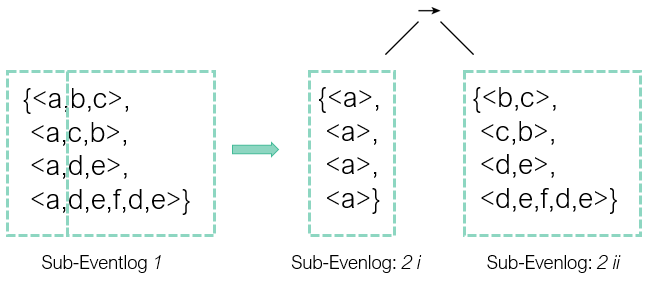
\includegraphics[scale=0.5]{figures/Appbildungen/im_example.PNG}
    \caption{Beispiel einer Trennung eines Eventlogs nach dem Inductive Miner Verfahren}
    \label{fig:imExample}
\end{figure}

Mehrere Varianten des Inductive Miners sind entwickelt worden, die das hier vorgestellte Verfahren erweitern. Sie werden entwickelt, um bestimmte Schwächen des Verfahrens zu umgehen oder den Algorithmus für spezifische Anwendungsfälle anzupassen. 
Beispielsweise kann das Protokoll selten auftretendes, aber für den Kontext wichtiges Verhalten enthalten, was Algorithmen zwingt, diese Einträge entweder auszuschließen oder komplizierte, unlesbare Modelle auszugeben, die jeden beliebigen Prozess beschreiben, also in einem  Blumenmodell wie in Appbildung \ref{fig:exampleFlower} entsprechen. Um dieses Problem schnell und effektiv zu lösen ist der Inductive Miner infrequent, kurz IMf\cite{inducFMining} entwickelt worden.

Eine anderes Problem, welches häufig auftritt, ist ein Protokoll das unzureichende Informationen enthält, um ein Prozessmodell zu finden, das das System gut repräsentiert. Unvollständigkeit zwingt Algorithmen, entweder das fehlende Verhalten auszuschließen und damit das noch unsichtbare Verhalten zu reduzieren, das das Modell erzeugen kann, oder das fehlende, unbekannte Verhalten dort einzubeziehen, indem sie das Risiko eingehen, falsch zu raten. Im Hinblick auf diese Problematik ist der Inductive Miner incomplete, kurz IMc \cite{inducIMining} entstanden.

\subsection{Local Process Miner}
Der Local Process Miner ist eines der jüngsten Verfahren der Discovery Process Miner, es wurde 2016 im 'Journal of Innovation in Digital Ecosystems' vorgestellt \cite{localMining}. Local Process Mining basiert auf den Erkenntnissen aus der Entwicklung des Sequential Pattern Mining\cite{Srikant1996MiningSP} und des Episode Mining \cite{mannila1997discovery}.

Der Local Process Miner unterscheidet sich von den anderen, hier vorgestellten Algorithmen, dadurch, dass er nicht ein, sondern mehrere Modelle erzeugt. Die Modelle beschreiben dabei häufiges, aber partielles Verhalten und bestehen dabei aus nicht mehr als drei bis fünf Knoten. Das heißt jedes einzelne der entstandenen Netze modelliert nur eine Teilmenge der Aktivitäten, die im Ereignisprotokoll beobachtet werden. 

Der Algorithmus lässt sich in vier iterativen Schritten zusammenfassen, der initialen Generation, der Evaluation, der Selektion und der Expansion. LPM arbeitet auf sogenannten Process Trees auf, der Prozess wird also als Baumstruktur beschrieben. Die  Kindknoten des Baumes werden als Nachfolger von Elternknoten abstrahiert, die Knoten repräsentieren, wie beim Petri Netz auch, einzelne Ereignisse beziehungsweise Einträge eines Eventlogs oder Übergänge zwischen den Einträgen. 

Zunächst wird eine Menge von einblättrigen Prozessbäumen $CM_1$, $i=1$ generiert, jedes Blatt entspricht einem Eintrag des zu analysierenden Eventlogs. Die gegebene Menge wird nach vordefinierten Qualitätskriterien evaluiert. Auf Basis der Evaluation wird eine Teilmenge $SCM_i \subseteq CM_i$ ausgewählt. In diesem Schritt prüft die Abbruchbedingung, ob die nutzerdefinierte maximale Anzahl an Iterationsschritten erreicht wurde oder die Teilmenge $SCM_i=∅$  ist. Wird eine der beiden Bedingungen erfüllt, endet der Algorithmus. Werden sie nicht erfüllt, folgt Schritt vier, die Expansion. 

In jedem Expansionsschritt wird die Menge aus einzelnen Prozessbäume zu einer Menge aus größeren Bäumen $CM_i+1$ erweitert. Bei der Expansion wird jeder Knoten ersetzt durch einen Sub-Prozessbaum, der diesen Knoten enthält. Beispielsweise ist eine mögliche Erweiterung von $a$: $ →(a,b)$, die als neues Element der Menge $CM_2$ deklariert wird, wie in Abbildung \ref{fig:lpmExample} zu sehen ist. 
\begin{figure}[!h]
    \centering
    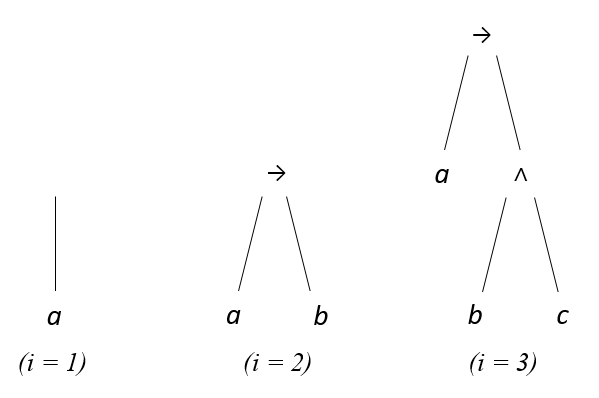
\includegraphics[scale=0.45]{figures/Appbildungen/lpm_example.PNG}
    \caption{Ein initialer Prozessbaum und seine Expansion im Local Process Miner, (Eigene Darstellung in Anlehnung an: Dalmas B., N. Tax, 2017, S.5, \cite{lpm}) }
    \label{fig:lpmExample}
\end{figure}

An den Expansionsschritt knüpft wieder ein Selektionsschritt an, die Selektion erfolgt über eine Reihe von für den gegebenen Eventlog berechneten Schwellwerten, Vgl. \cite{lpm}. Die resultierenden Prozessbäume können abschließend in Petri Netze überführt werden.

Die für das Local Process Mining charakteristischen kurzen Ausgangsmodelle sind nicht, oder nur unzureichend, geeignet, um dem Anwender einen Eindruck von langkettigen Prozessen zu verschaffen und Prozesse grob zu abstrahieren. Allerdings sind die Ausgangsmodelle besser geeignet als andere gängige Process Mining Algorithmen, Detailansichten von Prozessen zu konstruieren. 
Diese können je nach Anwendungsfall besonders hilfreich sein, um festzustellen welche kleinschrittigen Muster und Routinen sich in einem Prozess verbergen, die von Ausgabemodellen, die einen Prozess vollständig abdecken wollen, häufig übergangen werden. Allerdings ist dieses Verfahren bisher sehr rechenintensiv, was auch darauf zurück zu führen ist, dass seit seiner Veröffentlichung nicht genug Zeit vergangen ist, um auf seine Rechenzeit hin optimiert zu werden.

%Die Wahl eines Verfahrens sollte entsprechend nicht allein darauf beruhen, evtl. mehr bla bla 

\section{Protokolldateien}
\subsection{Tabellarische Eventlogs}
Nachdem im vorangegangenem Kapitel auf die verschiedenen Prozess Mining Algorithmen eingegangen wurde, sollen in diesem Kapitel die, allen Verfahren gemeinen, Ein- und Ausgangsdaten näher betrachtet werden.
In praktischen Anwendungen liegen die Eingangsdaten in der Regel als Protokolldateien vor. Die Beschaffenheit der in dieser Arbeit verwendeten  Protokolldateien, die als Basis für die die Analyse und letztendliche Erzeugung von Petri Netzen dienen, soll hier wieder anhand eines Beispiels beschrieben werden.

Um einen Prozess basierend auf einer Protokolldatei erkennen zu können, muss die Datei zunächst einem formalen Schema folgen. Es können der Zeitstempel des Eintrags, die Ressource, die den Eintrag einleitet, sowie signifikante Eigenschaften der jeweiligen Ressource, wie den Zustand oder die Lokalisation enthalten, in der Protokolldatei vorliegen.

Tabelle \ref{tab:example-Eventlog} zeigt ein fiktives Protokoll, welches auch Teil der nachfolgenden Versuchsreihe ist. 
\begin{table}[!ht]
\centering
\resizebox{260pt}{!}{%
\begin{tabular}{l|lll}
\textbf{case} & \textbf{timestamp} & \textbf{resource} & \textbf{activity} \\ \hline
AA & 2019-01-01 07:36:36 & Coffee maker & turned to ON \\
AA & 2019-01-01 07:38:03 & Appliance g & read 0 \\
AA & 2019-01-01 07:42:09 & Doorbell & ringing \\
AA & 2019-01-01 07:45:36 & Coffee maker & Two Esprosso Cups \\
AA & 2019-01-01 07:45:42 & Appliance b & read 90 \\
... & ... & ... & ... \\ \hline
AB & 2019-01-02 07:33:27 & Doorbell & ringing \\
AB & 2019-01-02 07:35:51 & Coffee maker & turned to ON \\
AB & 2019-01-02 07:35:57 & Appliance j & read 90 \\
AB & 2019-01-02 07:36:15 & Appliance h & read 67 \\
AB & 2019-01-02 07:42:27 & Coffee maker & Two Esprosso Cups \\
... & ... & ... & ... \\ \hline
AC & 2019-01-03 07:34:30 & Doorbell & ringing \\
AC & 2019-01-03 07:36:54 & Coffee maker & turned to ON \\
AC & 2019-01-03 07:38:21 & Appliance c & read 45 \\
AC & 2019-01-03 07:39:06 & Appliance g & read 13 \\
AC & 2019-01-03 07:43:30 & Coffee maker & Two Esprosso Cups \\
... & ... & ... & ... \\ \hline
AD & 2019-01-04 07:35:33 & Doorbell & ringing \\
AD & 2019-01-04 07:35:57 & Appliance h & read 90 \\
AD & 2019-01-04 07:37:57 & Coffee maker & turned to ON \\
AD & 2019-01-04 07:41:30 & Appliance f & read 67 \\
AD & 2019-01-04 07:43:30 & Coffee maker & Two Esprosso Cups \\
... & ... & ... & ... \\ \hline
\end{tabular}%
}
\caption{Auszug aus Eventlog der Versuchsreihe in Kapitel \ref{chap:approach}}
\label{tab:example-Eventlog}
\end{table}
Eine grundlegende Annahme der Process Mining Verfahren ist, dass die Ereignisse eines Protokolls alle Teil eines zusammenhängenden Prozesses sind. Weiterhin entspricht jeder Eintrag, oder eine Zeile in der Tabelle, jeweils genau einem atomaren Ereignis. Ereignisse die zu einer Prozessinstanz gehören müssen alle mit dem selben sogenannten \textbf{Case} deklariert werden, eine Prozessinstanz bezeichnet einen isolierten Vorgang innerhalb eines Prozesses und kann aus einem oder mehreren Ereignissen bestehen. In Tabelle \ref{tab:example-Eventlog} entspricht ein Case jeweils dem Zeitraum von einem Kalendertag, Cases können auch danach differenziert werden, welche Person mit einem Prozess assoziiert wird, oder beispielsweise bei Supportanfragen über die ID des gemeldeten Vorfalls differenziert werden.

Es wird weiterhin mindestens eine Spalte, genannt \textbf{Activity}, benötigt, welche beschreibt, um welche Aktion es sich bei dem aufgenommenen Ereignis handelt. Activities stehen nie für sich allein,  sondern gehören immer zu einer sogenannten \textbf{Ressource}, die für die Erzeugung des Eintrags verantwortlich ist. Beispielsweise werden gemessene Sensorwerte (Activity) immer mit der Bezeichnung des Sensors (Ressource) eingetragen, Aktionen die von Personen durchgeführt wurden können die Person als Ressource identifizieren.

Die sequentielle Abfolge der Einträge ist besonders relevant für die Auswertung der Protokolldatei. Liegen neben der Aktivität zur Ressouce auch Zeitstempel, englisch \textbf{Timestamp}, vor, können diese bei der Auswertung zusätzlich berücksichtigt werden, dann fließt die zeitliche Distanzen als Metrik in die Auswertung mit ein. Fehlen Zeitstempel, so wird angenommen, dass die Distanzen zwischen einzelnen Ereignissen mit dem gleicen Wert gewichtet werden können.
Jede weitere Spalte, die Metainformationen liefert, kann die Ausgabequaltät zusätzlich verbessern. Diese Spalten werden auch als die Attribute des Ereignisses bezeichnet. 

\subsection{XES Standard}
Um Ereignisprotokolle einheitlich und herstellerunabhängig mit verschiedenen Werkzeugen verarbeiten zu können, wurde 2004 die Mining eXtensible Markup Language (MXML) definiert. Sie wurde durch das eXtensible Event Stream(XES) Format abgelöst \cite{xesmxml} und ist 2016 von der 'IEEE Task Force on Process Mining' als Standard anerkannt worden. 

Ein XES Dokument enthält jeweils eine Protokolldatei mit einer beliebigen Anzahl an Ereignissen, in einer festen Abfolge, und beliebig vielen Attributen, die vom Typ, wie beim zugrundeliegenden XML Standard auch, String, Date, Int, Float oder Boolean sein können. 
Der Anwender kann Attribute als erforderlich deklarieren, eigene Attribute definieren oder auf die vom XES Modell definierten Typen zugreifen. XES  wird von einer weiten Bandbreite an Process Mining Software unterstützt und zählt gemeinhin als favorisiertes Datenformat für die Verarbeitung durch Process Mining Algorithmen hin zu Process Modellen.

Konvertiert man das Ereignisprotokoll aus Tabelle \ref{tab:example-Eventlog} in ein XES Dokument erhält man eine Datei mit einer Struktur wie in Auszug 2.1:

\lstset{language=XML}
\begin{lstlisting}[label=lst:xes,caption=Auszug aus XES Datei zu Eventlog in Tabelle 2,captionpos=b]
<?xml version="1.0" encoding="UTF-8" ?>
    <!-- XES standard version: 1.0 -->
    <!-- OpenXES library version: 1.0RC7 -->
    <!-- OpenXES is available from http://www.openxes.org/ -->
    <Eventlog xes.version="1.0" xes.features="nested-attributes" openxes.version="1.0RC7">
    	<extension name="Lifecycle" prefix="lifecycle"/>
    	<extension name="Time" prefix="time"/>
    	<extension name="Concept" prefix="concept"/>
    	<classifier name="Event Name" keys="concept:name"/>
    	<string key="concept:name" value="XES Event Eventlog"/>	<trace>
		<string key="concept:name" value="AA"/>
		<event>
			<string key="resource" value="Doorbell"/>
			<string key="lifecycle:transition" value="start"/>
			<string key="concept:name" value="Doorbell ringing"/>
			<date key="time:timestamp" value="2019-01-01T07:32:24.000+02:00"/>
			<int key="Event ID" value="100"/>
		</event>
		<event>
			<string key="resource" value="Appliance c"/>
			<string key="lifecycle:transition" value="start"/>
			<string key="concept:name" value="Appliance r read 44"/>
			<date key="time:timestamp" value="2019-01-01T07:32:48.000+02:00"/>
			<int key="Event ID" value="101"/>
		</event>
\end{lstlisting}